\documentclass[aspectratio=169, table]{beamer}

%\usepackage[beamertheme=./praditatheme]{Pradita}
\usepackage[utf8]{inputenc}
\usepackage{xcolor} % for color
\usepackage{colortbl} % for table color
\usepackage{listings}

% Define Java language style for listings
\lstdefinestyle{JavaStyle}{
language=Java,
basicstyle=\ttfamily\tiny,
keywordstyle=\color{blue},
commentstyle=\color{gray},
stringstyle=\color{red},
breaklines=true,
showstringspaces=false,
tabsize=2,
captionpos=b,
numbers=left,
numberstyle=\tiny\color{gray},
frame=lines,
backgroundcolor=\color{lightgray!10},
comment=[l]{//},
morecomment=[s]{/*}{*/},
commentstyle=\color{gray}\ttfamily,
string=[s]{'}{'},
morestring=[s]{"}{"},
%	stringstyle=\color{teal}\ttfamily,
%	showstringspaces=false
}

\lstdefinestyle{sql}{
language=sql,
keywords={use, insert, into, values, select, from,
update, set, delete, create, where, join, left, right, inner, order, by, primary, key},
ndkeywords={max, min, varchar, int},
ndkeywordstyle=\color{purple}\bfseries,
basicstyle=\ttfamily\scriptsize,
keywordstyle=\color{blue},
commentstyle=\color{gray},
stringstyle=\color{red},
breaklines=true,
showstringspaces=false,
tabsize=2,
captionpos=b,
numbers=left,
numberstyle=\tiny\color{gray},
frame=lines,
backgroundcolor=\color{lightgray!10},
comment=[l]{\#},
morecomment=[s]{/*}{*/},
commentstyle=\color{gray}\ttfamily,
string=[s]{'}{'},
morestring=[s]{"}{"},
%	stringstyle=\color{teal}\ttfamily,
%	showstringspaces=false
}

\lstdefinelanguage{bash} {
keywords={},
basicstyle=\ttfamily\scriptsize,
keywordstyle=\color{blue}\bfseries,
ndkeywords={iex},
ndkeywordstyle=\color{purple}\bfseries,
sensitive=true,
commentstyle=\color{gray},
stringstyle=\color{red},
numbers=left,
numberstyle=\tiny\color{gray},
breaklines=true,
frame=lines,
backgroundcolor=\color{lightgray!10},
tabsize=2,
comment=[l]{\#},
morecomment=[s]{/*}{*/},
commentstyle=\color{gray}\ttfamily,
stringstyle=\color{purple}\ttfamily,
showstringspaces=false
}

\lstdefinestyle{XmlStyle} {
language=xml,
keywords={xmlns,version,type,import},
basicstyle=\ttfamily\scriptsize,
keywordstyle=\color{blue}\bfseries,
ndkeywords={import},
ndkeywordstyle=\color{purple}\bfseries,
sensitive=true,
commentstyle=\color{gray},
stringstyle=\color{red},
numbers=left,
numberstyle=\tiny\color{gray},
breaklines=true,
frame=lines,
backgroundcolor=\color{lightgray!10},
tabsize=2,
showstringspaces=false,
comment=[l]{\#},
commentstyle=\color{gray}\ttfamily,
stringstyle=\color{purple}\ttfamily,
morecomment=[s]{<!--}{-->}
}

\lstdefinelanguage{css}{
basicstyle=\ttfamily\footnotesize,
keywordstyle=\color{blue},
commentstyle=\color{gray},
stringstyle=\color{red},
breaklines=true,
showstringspaces=false,
tabsize=2,
captionpos=b,
numbers=left,
numberstyle=\tiny\color{gray},
frame=lines,
backgroundcolor=\color{lightgray!10},
comment=[l]{//},
morecomment=[s]{/*}{*/},
commentstyle=\color{gray}\ttfamily,
string=[s]{'}{'},
morestring=[s]{"}{"},
%	stringstyle=\color{teal}\ttfamily,
%	showstringspaces=false
}

\lstdefinelanguage{puml}{
	basicstyle=\ttfamily\footnotesize,
	keywords={@startuml, @enduml, class, String, abstract, interface, Person, note, of, end, enum},
	ndkeywords={right, left},
	morekeywords={\{,\}, <!-- },
	emph={=,!,?}, emphstyle=\color{red}\bfseries,
	keywordstyle=\color{blue},
	commentstyle=\color{gray},
	stringstyle=\color{teal},
	ndkeywordstyle=\color{purple}\bfseries,
	breaklines=true,
	showstringspaces=false,
	tabsize=2,
	captionpos=b,
	numbers=left,
	numberstyle=\tiny\color{gray},
	frame=lines,
	backgroundcolor=\color{lightgray!10},
	comment=[l]{\'},
	morecomment=[s]{/*}{*/},
	commentstyle=\color{gray}\ttfamily,
	%	string=[s]{'}{'},
	morestring=[s]{"}{"},
	%	stringstyle=\color{teal}\ttfamily,
	%	showstringspaces=false
	literate=
	{\{}{{\textcolor{red}{\{}}}1
	{\}}{{\textcolor{red}{\}}}}1
	{:}{{\textcolor{red}{:}}}1
	{=}{{\textcolor{red}{=}}}1
}

\usetheme{Pradita}

\subtitle{IF220303 - Object-oriented Programming}

\title{\LARGE{Unified Modeling Language:}\\\LARGE{Behavioral Diagrams}\vspace{20pt}}
\date[Serial]{\scriptsize {PRU/SPMI/FR-BM-18/0222}}
\author[Pradita]{\small {\textbf{Alfa Yohannis}}}

\begin{document}

\frame{\titlepage}

\begin{frame}[fragile]
\frametitle{Contents}
\vspace{10pt}
\begin{columns}[t]
	\column{0.5\textwidth}
	\tableofcontents[sections={1-5}]
	
	\column{0.5\textwidth}
	\tableofcontents[sections={6-10}]
\end{columns}
\end{frame}

\section{Behavioral Diagram}

\begin{frame}[fragile]{Behavioral Diagram}
	\vspace{20pt}
	\begin{columns}[t]
		\column{0.5\textwidth}
		\textbf{Behavioral diagram} is a type of diagram in the \textit{Unified Modeling Language} (UML) used to:
		\begin{itemize}
			\item Represent the dynamics and interactions within a software system.
			\item Illustrate how components in the system operate.
			\item Show the flow of data or information within the system.
			\item Visualize object interactions during execution.
		\end{itemize}
		
		\column{0.5\textwidth}
		\textbf{Benefits of Behavioral Diagrams:}
		\begin{itemize}
			\item Understand the system workflow before implementation.
			\item Assist in requirements analysis and software design.
		\end{itemize}
		
		\textbf{Types of Behavioral Diagrams in UML:}
		\begin{itemize}
			\item Sequence Diagram
			\item Activity Diagram
			\item State Machine Diagram
			\item Use Case Diagram
		\end{itemize}
	\end{columns}
\end{frame}


\begin{frame}{Activity}
	\framesubtitle{Diagram}
	\centering
	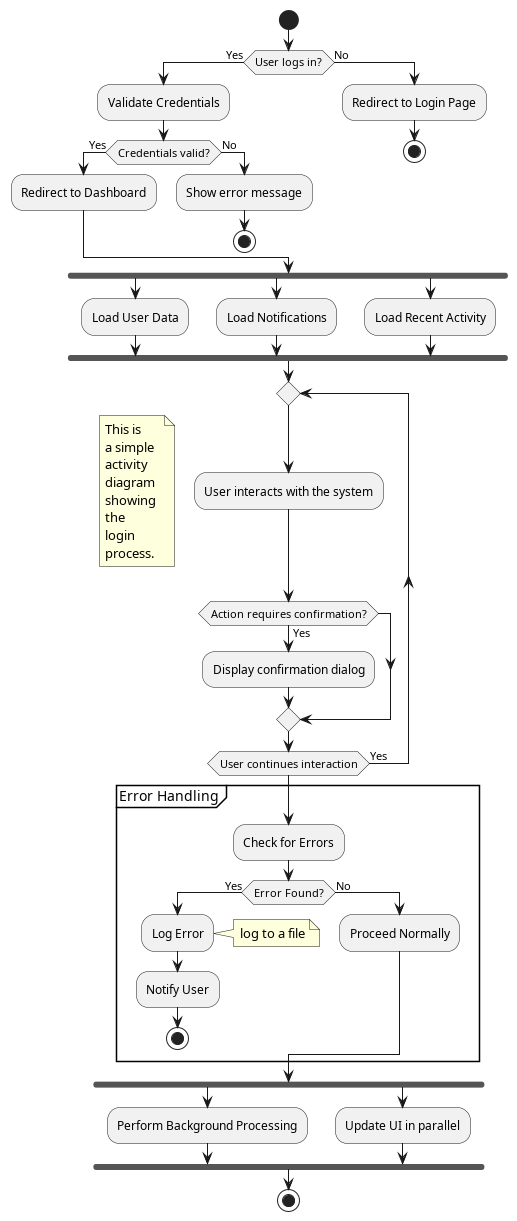
\includegraphics[width=\textwidth,height=0.97\textheight,keepaspectratio]{../../figures/out/activity_diagram.png}
\end{frame}

\begin{frame}{Sequence}
	\framesubtitle{Diagram}
	\centering
	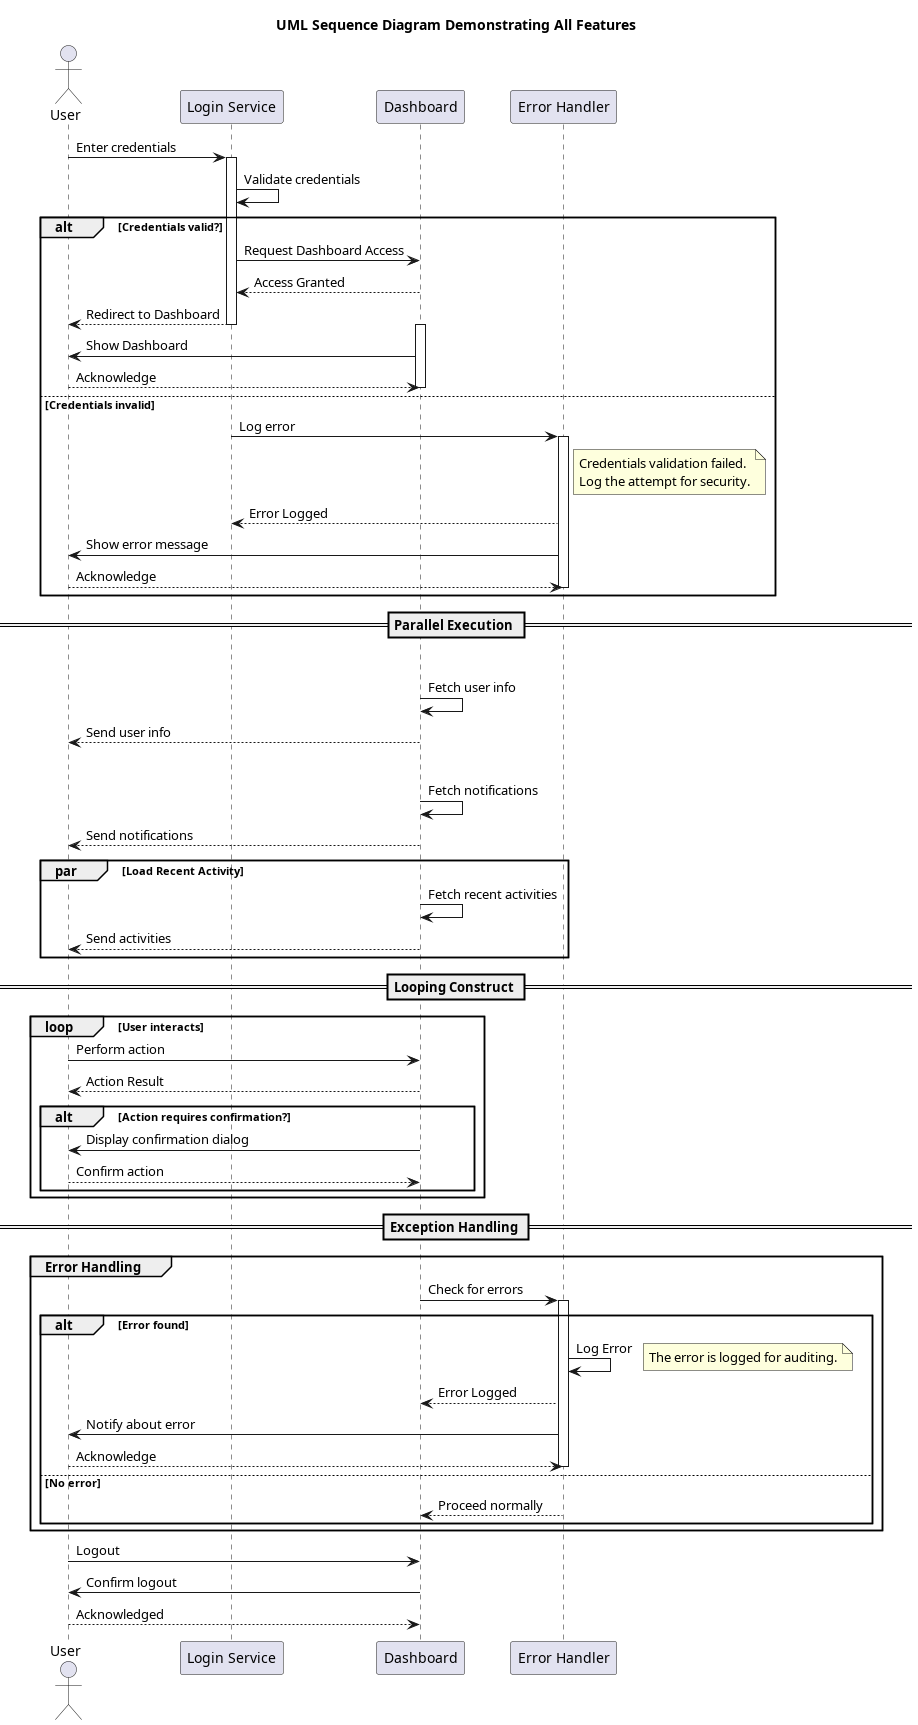
\includegraphics[width=\textwidth,height=0.97\textheight,keepaspectratio]{../../figures/out/sequence_diagram.png}
\end{frame}

\begin{frame}{Statechart Diagram}
	\vspace{30pt}
	\centering
	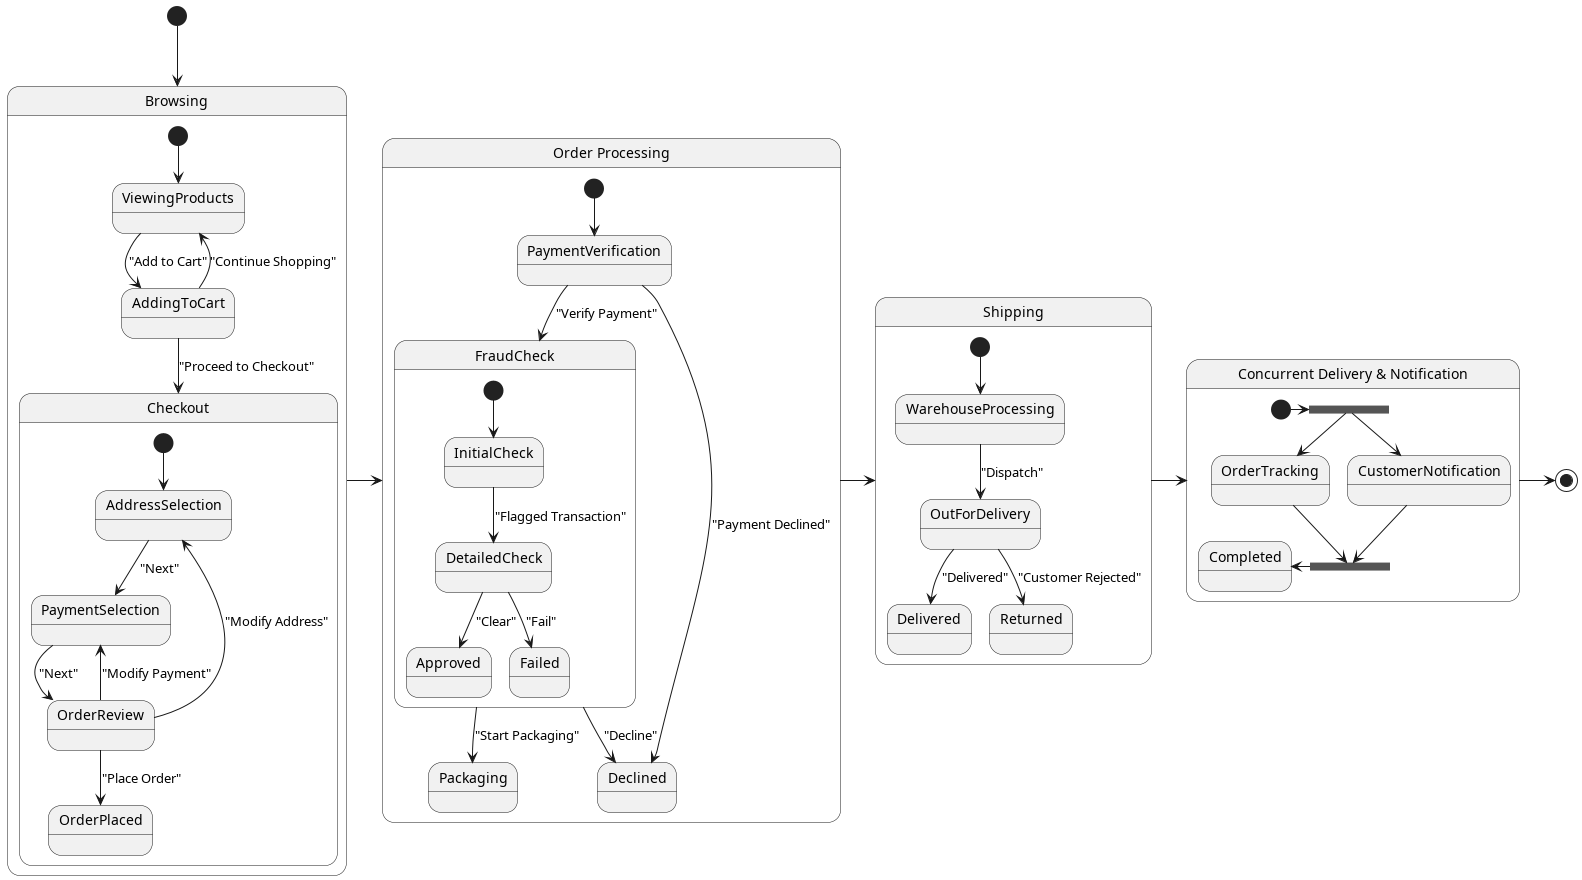
\includegraphics[width=\textwidth,height=0.8\textheight,keepaspectratio]{../../figures/out/statechart_diagram.png}
\end{frame}

\begin{frame}{Use Case Diagram}
	\vspace{30pt}
	\centering
	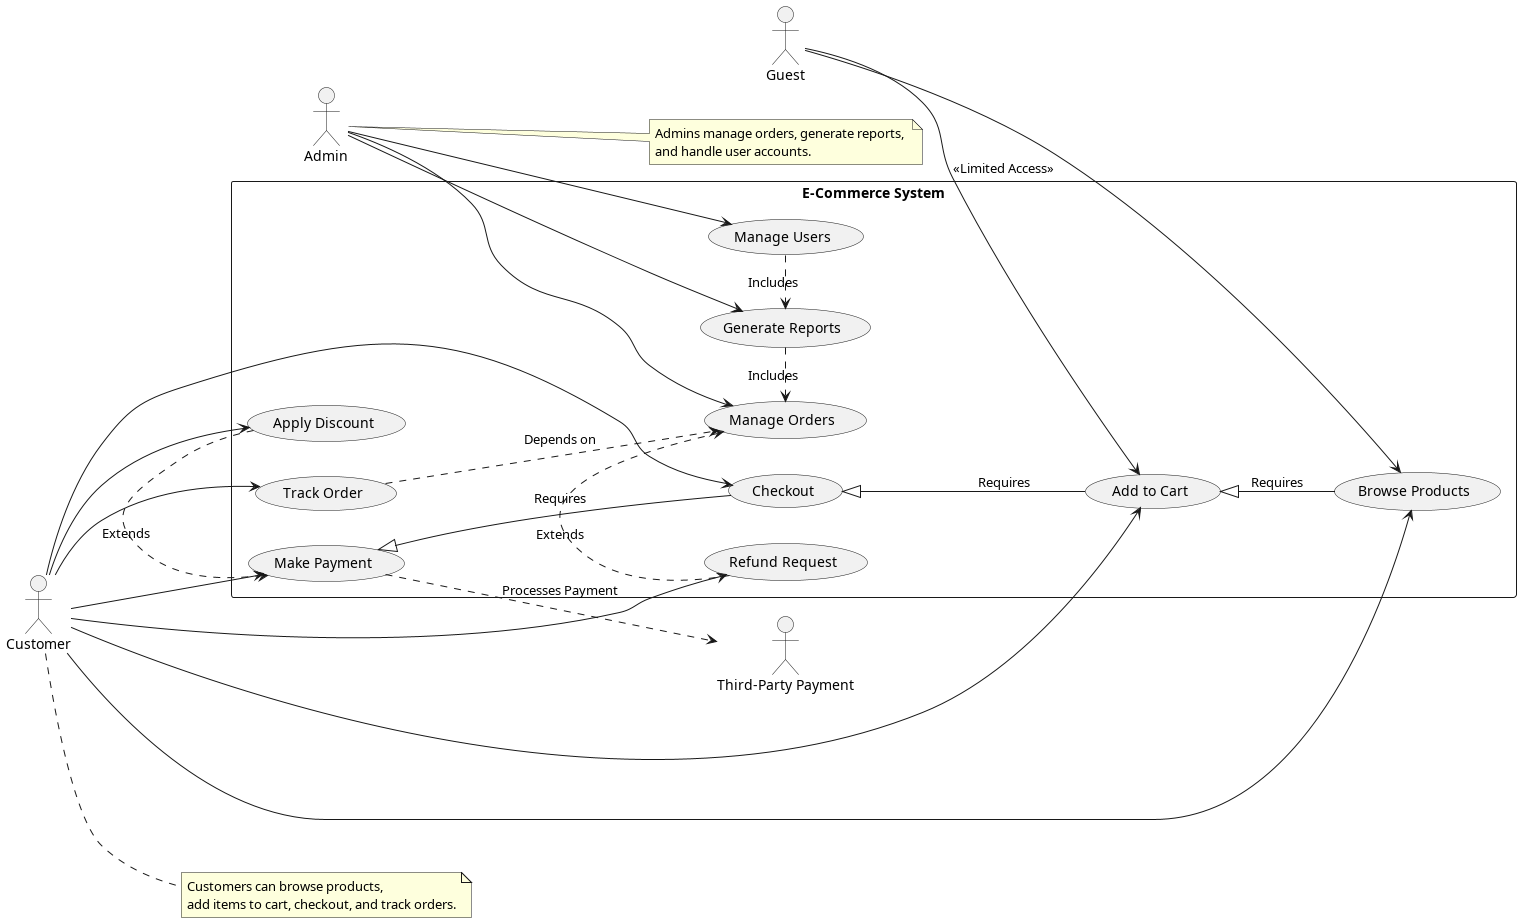
\includegraphics[width=\textwidth,height=0.8\textheight,keepaspectratio]{../../figures/out/usecase_diagram.png}
\end{frame}

\section{References}

\begin{frame}{References}
	\vspace{20pt}
	For a more in-depth study of UML, please visit the following link:  
	\url{https://www.uml-diagrams.org/}
\end{frame}


\end{document}
